\documentclass{scrbook}
\usepackage{graphicx} % Required for inserting images
\usepackage{tabularx} % Required for fixed width tables
\usepackage{scrlayer-scrpage} % Required for the subtitles
\usepackage{url} % Required for the URLs
\usepackage{hyperref} % Required for the URLs
\usepackage{listings} % Required for the code snippets
\usepackage{mathtools} % Required for the system of equations
\usepackage{amsmath,amssymb} % Required for some math symbols
\usepackage{enumitem} % Required for lettered lists

% Put the caption of the snippets at the bottom
\lstset{
    captionpos=b
}


\title{Web browser}
\subtitle{Ambient intelligence course (A.Y. 2025/2026)\\Topic taught by Prof. Floriano Scioscia}
\author{Gabriele Colapinto}
\date{\today}

\begin{document}

\maketitle
\thispagestyle{empty}

{\Large\textbf{License}} \\
{Notes from Ambient intelligence (A.Y. 2025/2026) by Gabriele Colapinto. 
Course taught by professors Michele Ruta, Floriano Scioscia, Arnaldo Tomasino, Davide Loconte — 
Licensed under CC BY-NC 4.0.\\
\url{https://creativecommons.org/licenses/by-nc/4.0/}}

\vspace*{\fill}
\rule{\textwidth}{0.2pt}
\small{© 2025 Gabriele Colapinto \\
Released under the \href{https://creativecommons.org/licenses/by-nc/4.0/}{Creative Commons Attribution–NonCommercial 4.0 International License}}

\clearpage

\tableofcontents

\chapter{Introduction: Defining the Web Browser}

Understanding the modern web browser is fundamental to engaging with nearly all web-oriented technologies. As the primary user agent for interacting with web content, the browser has evolved from a simple document viewer into a sophisticated application platform. It serves as the critical bridge between remote information stored on web servers and the end-user's device, making its architecture a key area of study for anyone involved in web development or systems design. \\

At its core, a web browser is a software program designed to retrieve, interpret, and display documents and other resources from the World Wide Web. It acts on behalf of a user to request content from a server—identified by a Uniform Resource Locator (URL)—and then renders that content visually, typically within a window on the user's screen. While this definition captures its primary purpose, the functionalities of a modern browser extend far beyond simple retrieval and display. \\

The core functionalities of a typical web browser include:

\begin{itemize}
    \item \textbf{Resource Handling:} Displaying web resources, such as HTML pages, directly within its own window or passing specific file types to external helper applications for processing.
    \item \textbf{Navigation:} Retrieving resources either through the user's direct specification of a URL or by following hyperlinks embedded within other documents—the foundational mechanism of the web.
    \item \textbf{Session Management:} Tracking the user's navigation history to allow for easy backtracking and providing mechanisms for bookmarking pages of interest for quick recall.
    \item \textbf{Data Storage:} Storing user-provided information, such as values entered into web forms and account credentials for websites, to enhance user convenience and streamline subsequent interactions.
    \item \textbf{Accessibility:} Providing features to make web content usable for individuals with various disabilities, including blindness, low vision, and motor or hearing impairments.
\end{itemize}

These features, now standard in contemporary browsers, are the product of decades of technological evolution and competition, a history that has directly shaped the complex systems we use today.

\chapter{A History of Innovation and Competition}

To understand the architecture of modern web browsers, it is essential to appreciate their history. This evolution, marked by periods of intense competition and collaborative standardization, has directly forged the web technologies and architectural patterns in use today. From the first simple graphical viewers to today's complex application platforms, the browser's history is a story of strategic innovation that continues to define the digital landscape.

\section{The Pioneers: From Berners-Lee to Mosaic}

The genesis of the web browser is directly linked to the invention of the World Wide Web itself. In 1991, Tim Berners-Lee, while at CERN, developed the first web browser as a demonstration of the web technologies he had proposed: HTML, URLs, and HTTP. This initial program was not just a viewer; it also functioned as an HTML editor, addressing the practical need to create content for the new medium. \\

However, the web's explosion in popularity began with the release of NCSA Mosaic in 1993. Developed at the National Center for Supercomputing Applications, Mosaic was the first browser to allow images to be embedded directly within the text of a web page, rather than appearing in a separate window. This feature was a critical factor in transforming the web from a text-based academic tool into a visually engaging medium for the general public. The technology was later commercialized through a company called Spyglass, marking the first major step toward a commercial web.

\section{The Browser Wars: Netscape vs. Internet Explorer}

The commercial potential of the web, demonstrated by Mosaic, led directly to the first "browser war." A primary developer of Mosaic left NCSA to co-found Netscape, which released its own highly successful browser. Recognizing the strategic importance of this emerging platform, Microsoft entered the market in 1995 with Internet Explorer, a browser initially based on code licensed from Spyglass. \\

What followed was a period of intense competition for market dominance between Netscape and Internet Explorer. Microsoft ultimately emerged victorious, partly through its business practices but also through its technical strategy. A key tactic was to adopt the standards proposed by the World Wide Web Consortium (W3C) in an incomplete or incompatible manner while simultaneously introducing proprietary, non-standard technologies. Features like VBScript and ActiveX were designed to create vendor lock-in, encouraging developers to build web applications that worked exclusively, or best, on Internet Explorer. This approach fragmented the web and created significant challenges for cross-browser compatibility that would persist for years.

\section{The Rise of Open Source and Modern Browsers}

The end of the first browser war had a profound impact on the web's trajectory. In 1998, with its market share collapsing, Netscape made a pivotal decision: it released its browser's source code to the public, leading to the creation of the open-source Mozilla Foundation. This foundation would later develop Firefox, a standalone browser that successfully clawed back significant market share from Internet Explorer and championed web standards. \\

This period also saw the rise of the "software fork," where developers take an existing open-source codebase and start independent development. The web browser space provides a prime example of this pattern. The core components of the open-source Konqueror browser were forked by Apple to create WebKit, the rendering engine for its Safari browser. Later, Google forked WebKit to create Blink, the engine that now powers Google Chrome. \\

Google Chrome's introduction in 2008 was another transformative moment. It was architected to solve three critical problems that had emerged from the browser wars and Internet Explorer's dominance:

\begin{enumerate}
    \item \textbf{Adherence to Web Standards:} Chrome was built with W3C standards compliance as a core principle, directly contrasting with Internet Explorer's reliance on proprietary features.
    \item \textbf{Security:} Recognizing the growing threat of malicious web content, Chrome introduced a novel multi-process architecture. By running each browser tab in a separate process, it ensured that a crash or security breach in one tab would not affect the others, significantly enhancing stability and security.
    \item \textbf{JavaScript Performance:} As web applications grew more complex ("Rich Internet Applications"), the performance of JavaScript, which was a purely interpreted language at the time, became a major bottleneck. Chrome introduced the V8 JavaScript engine, which featured just-in-time (JIT) compilation, dramatically increasing execution speed and enabling a new generation of powerful web applications.
\end{enumerate}

Today, the browser market is dominated by Chrome and its underlying open-source project, Chromium. This dominance has, ironically, led to the re-emergence of challenges similar to those of the Internet Explorer era, such as the introduction of proprietary APIs before they are standardized. In a significant market shift, Microsoft eventually abandoned its proprietary browser architecture and rebuilt its Edge browser on the Chromium codebase, solidifying the influence of this open-source project. \\

This dynamic history of competition and innovation drove the need for a more structured, modular approach to browser design, leading to the sophisticated architectures found in modern browsers.

\begin{figure}
    \centering
    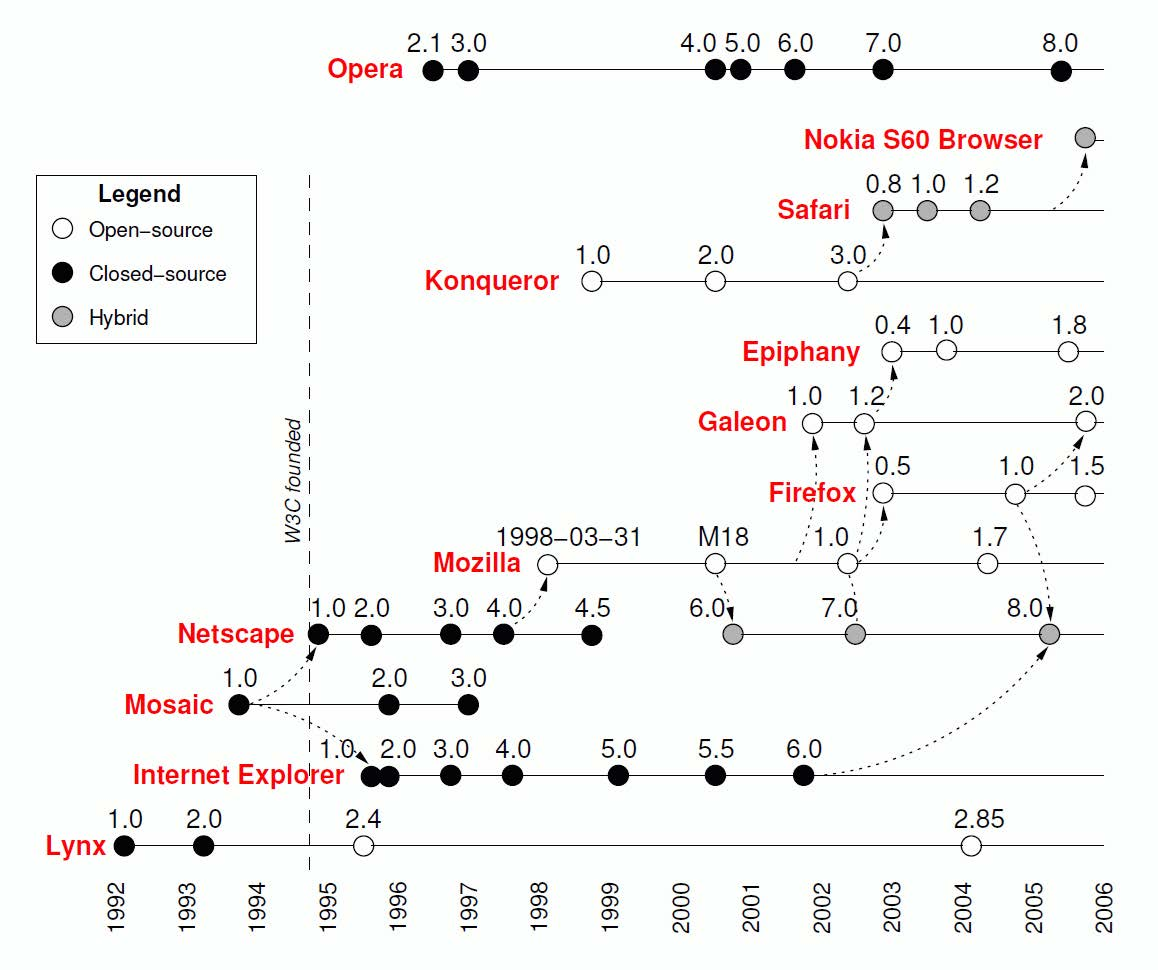
\includegraphics[width=\linewidth]{Images/Web_browser_timeline.jpg}
    \caption{Web browser timeline}
    \label{fig:web_browser_timeline}
\end{figure}

\chapter{The Architecture of a Modern Web Browser}

A modern web browser is a highly complex software system, composed of multiple interconnected components, each with a distinct responsibility. Far from being a monolithic application, its design reflects a modular architecture that can be understood using established software design patterns. This modularity allows for greater stability, security, and flexibility in adapting to the ever-changing web landscape.

\section{An Architectural Overview: The MVC Paradigm}

The general architecture of a web browser aligns well with the \textbf{Model-View-Controller (MVC)} software architectural pattern (See figure ~\ref{fig:web_browser_architecture}). MVC divides a program's logic into three interconnected elements, a separation that maps cleanly onto the primary functions of a browser:

\begin{itemize}
    \item \textbf{View:} The \textbf{User Interface (UI)} is the part of the browser the user directly interacts with. It is responsible for presenting information and accepting user commands.
    \item \textbf{Controller:} The \textbf{Browser Engine} acts as the central coordinator. It receives input from the UI (the View) and marshals actions to the appropriate backend component, primarily the Rendering Engine.
    \item \textbf{Model:} The \textbf{Rendering Engine} is responsible for managing the web content itself. It parses HTML and CSS to create an in-memory representation (the Model) of the web page, which is then displayed via the UI.
\end{itemize}

Beyond these three core elements, a browser's architecture includes several other major components that work in concert to deliver a complete web experience:

\begin{itemize}
    \item \textbf{Networking:} Handles all network communication, such as HTTP requests, to retrieve resources from servers.
    
    \item \textbf{JavaScript Interpreter:} Parses and executes JavaScript code embedded in web pages, enabling dynamic functionality.
    
    \item \textbf{Display Backend:} Provides the low-level drawing capabilities used by the Rendering Engine to paint pixels on the screen.
    
    \item \textbf{Data Persistence:} Manages the storage of user and session data on the local disk.

    \item \textbf{XML Parser:} Starting from a well-formed XML file it creates its tree structure representation, typically the DOM (Document Object Model). This component also check the correctness of the syntax of the document because, in case of malformed document, it returns a fatal error and the parsing fails.

    \item \textbf{HTML Parser:} Considering that the XML parser requires a well-formed document and the W3C decided to use a best-effort approach to the parsing of the HTML documents, browsers have another component to parse the web pages: the HTML parser (alas not shown in figure ~\ref{fig:web_browser_architecture}). This component not only parses the document to create its tree and DOM representation but also performs guesswork if necessary.
\end{itemize}

\begin{figure}
    \centering
    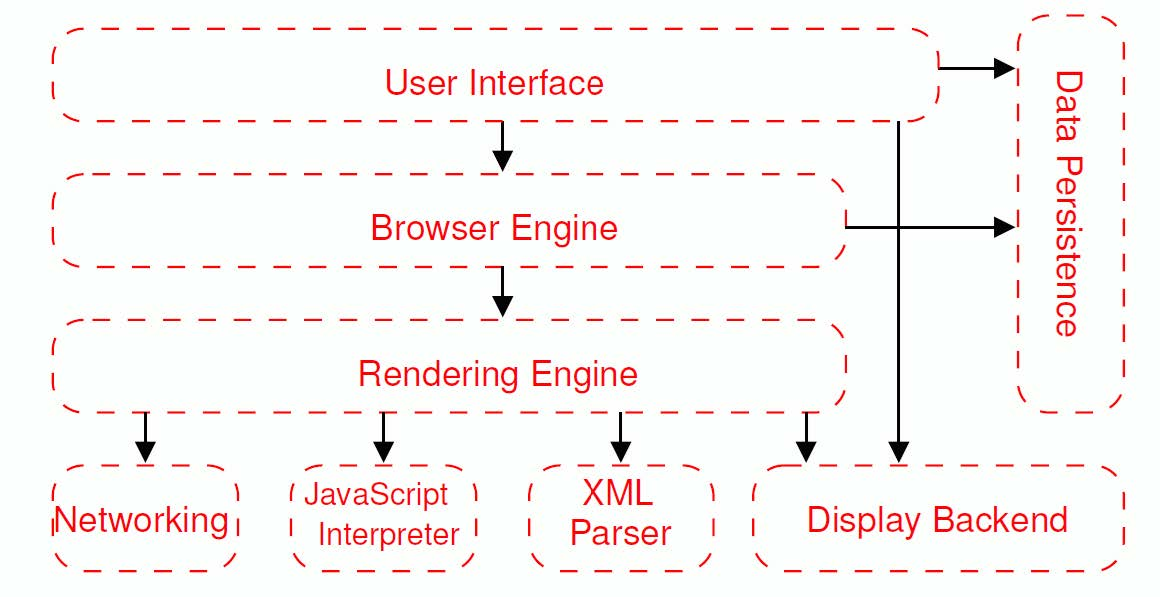
\includegraphics[width=\linewidth]{Images/Web_browser_architecture.jpg}
    \caption{Web browser architecture}
    \label{fig:web_browser_architecture}
\end{figure}

\section{The User Interface (UI)}

The User Interface (a.k.a. the chrome of the browser... and yes the browser by Google was named after this component) is the visual and interactive shell of the browser. It encompasses everything the user sees and interacts with that is not the web page content itself, including the main window frame, title bar, tabs, toolbars with navigation controls (like back, forward, and reload), the address bar, and menus for bookmarks and settings. \\

Recent decades have seen significant innovations in browser UI design. Key advancements include \textbf{tabbed navigation}, which allows users to manage multiple web pages within a single window, and \textbf{extensions}, a concept for which Firefox is directly credited with pioneering, enabling developers to add custom functionality and enhance the browser's UI. The design of the UI is not governed by any formal specification; rather, it evolves through established best practices in user experience (UX) design and a process of competitive imitation, where successful features introduced by one browser are often adopted by others.

\section{Data Persistence}

The data persistence component is responsible for managing all user-related data that needs to be stored locally between browsing sessions. This data can be categorized into two main types: high-level data that the user is actively aware of, and low-level data that is typically managed automatically by the browser.

\begin{table}[h]
    \centering
    \begin{tabular}{|l|l|}
    \hline
    \textbf{Data Type} & \textbf{Examples} \\
    \hline
    \textbf{High-Level Data} & Bookmarks, toolbar settings, saved form values, stored passwords. \\
    \hline
    \textbf{Low-Level Data} & Cookies, security certificates, cache. \\
    \hline
    \end{tabular}
    \caption{Data Types}
\end{table}

This component has undergone two major innovations to improve efficiency and functionality:

\begin{enumerate}
    \item \textbf{Embedded Databases:} Early browsers often stored data in proprietary flat-file structures. This approach was inefficient, making data access slow as the amount of information grew. Modern browsers have largely transitioned to using embedded databases like \textbf{SQLite}. This provides a more performant and open way to store and retrieve data using standard SQL queries.
    \item \textbf{Cloud Synchronization:} Modern browsers now offer the ability to synchronize user data across multiple devices. Information such as bookmarks, browsing history, saved passwords, and even the list of open tabs is encrypted and stored in the cloud, allowing a user to maintain a consistent browsing environment across their desktop computers and mobile devices.
\end{enumerate}

\section{The Browser Engine}

The Browser Engine serves as the core controller, coordinating operations between the User Interface and the Rendering Engine. It acts as the central hub for managing the browsing session. \\

Its primary functions include:

\begin{itemize}
    \item Initiating the loading of a resource specified by a URL.
    \item Handling high-level browsing actions initiated by the user via the UI, such as \texttt{reload}, \texttt{back}, and \texttt{forward}.
    \item Monitoring and reporting the progress of page loading to the UI.
\end{itemize}

Historically, the browser engine was also responsible for managing plugins—third-party, native-code libraries like Adobe Flash and Microsoft Silverlight that could be embedded in web pages to provide advanced interactivity. However, due to significant performance and security concerns—as these plugins greatly expanded the browser's attack surface—this approach has been phased out in favor of web-native technologies like HTML5 and JavaScript. The browser engine now orchestrates these modern, more secure technologies, with its most critical task being the management of the rendering engine.

\chapter{The Rendering Engine: From Code to Pixels}

The Rendering Engine is arguably the most critical component of a web browser, as it is responsible for the visual representation of all web content. Its fundamental role is to interpret code—primarily HTML and CSS—and translate it into the formatted, interactive layout that the user sees on their screen. From text and images to complex page structures, the rendering engine transforms abstract instructions into tangible pixels.

\section{The Role of the Rendering Engine}

The primary job of the rendering engine is to parse HTML and CSS documents to calculate the layout of a web page. This involves determining the size, position, and style of every element on the page. It is important to distinguish between the full page layout and the \textbf{viewport}. The viewport is the visible area of the browser window where content is displayed. While the user only sees the content within the viewport at any given moment, the rendering engine computes the layout for the entire page, including the parts that are currently off-screen. (See figure ~\ref{fig:viewport})\\

A key architectural innovation, pioneered by Google Chrome, is the \textbf{multi-process architecture}. In this model, the browser runs a separate instance of the rendering engine for each open tab, each in its own isolated process. This design provides significant benefits for both stability and security. If a rendering engine instance in one tab crashes due to a bug, it does not affect the other tabs or the main browser application. Similarly, this process isolation helps contain malicious code, preventing it from accessing data in other open pages.

\begin{figure}
    \centering
    
\includegraphics[width=0.5\linewidth]{Images/Viewport_in_web_page.png}
    \caption{Viewport in the web page}
    \label{fig:viewport}
\end{figure}

\section{The Document Object Model (DOM)}

The Document Object Model (DOM) is the central concept and data structure upon which all modern web page rendering and interactivity are built. It is the foundational in-memory representation of a web page that allows browsers and programming languages to understand and manipulate its content.

\subsection{Defining the DOM}

The DOM is a cross-platform and language-independent programming interface for HTML and XML documents. It provides a structured, object-oriented representation of a document's contents in the browser's memory. Instead of treating the document as a simple string of text, the DOM represents it as a logical tree of nodes and objects, where each object corresponds to a part of the document. This structure allows programs to programmatically access, navigate, and modify the content, structure, and style of the document.

\subsection{The DOM Tree Structure}

The logical structure created by the browser is known as the \textbf{DOM Tree}. This is a hierarchical representation of a document's contents, where the relationships between elements are defined in a parent-child structure. In this tree, every part of the document is a \textbf{node}:

\begin{itemize}
    \item The document itself is the root node.
    \item Every HTML element (e.g., \texttt{<body>}, \texttt{<h1>}, \texttt{<p>}) is an element node.
    \item The text contained within an element is a text node.
\end{itemize}

This tree structure accurately models the nested nature of HTML and provides a clear path for accessing any part of the document.

\subsection{The DOM as a Programming Interface}

The DOM is what enables dynamic, interactive web pages. While it is often discussed in the context of JavaScript, the DOM itself is not part of the JavaScript language. Instead, it is a Web API that JavaScript can use to interact with a web page. JavaScript acts as the scripting language that can "talk" to the DOM, using the API to perform actions such as:

\begin{itemize}
    \item Changing the text content of an element.
    \item Adding or removing elements from the page.
    \item Modifying the CSS styles of an element.
\end{itemize}

This powerful interface between a scripting language and the document's structure is the engine of all modern client-side web application functionality.

\section{The Rendering Pipeline in Detail}

The process of turning HTML and CSS code into visible pixels on the screen can be understood as a sequential pipeline executed by the rendering engine (See figure ~\ref{fig:rendering_engine_basic_flow}). This process involves several distinct stages:

\begin{enumerate}
    \item \textbf{HTML Parsing:} The process begins with the HTML parser, which processes the HTML markup from the server. As it parses the document, it constructs the \textbf{DOM Tree} in memory, creating the logical representation of the page's structure.
    
    \item \textbf{CSS Parsing:} Simultaneously, the CSS parser processes all associated stylesheets, including external CSS files and inline style tags. It parses this CSS into a data structure representing the style rules, which maps selectors to declarations of visual properties (e.g., color, size, position). This structure is then used in the next stage to style the document's elements.
    
    \item \textbf{Attachment/Render Tree Construction:} In this stage, the DOM tree and the style rules are combined. The engine traverses the DOM tree and, for each visible node, attaches the relevant style rules. The result is a new tree called the \textbf{Render Tree} (See figure ~\ref{fig:render_tree}), which contains only the visual information needed to display the page.
    
    \item \textbf{Layout:} The layout stage takes the render tree and calculates the exact coordinates for each node. This process, also known as "reflow," determines the precise position and size of every element within the viewport and the page as a whole.
    
    \item \textbf{Painting:} The final stage is painting. The rendering engine traverses the render tree and issues painting commands to a \textbf{display backend}. This backend component is responsible for using the operating system’s native graphical libraries to draw the pixels on the screen, bringing the webpage to life.
\end{enumerate}

\begin{figure}
    \centering
    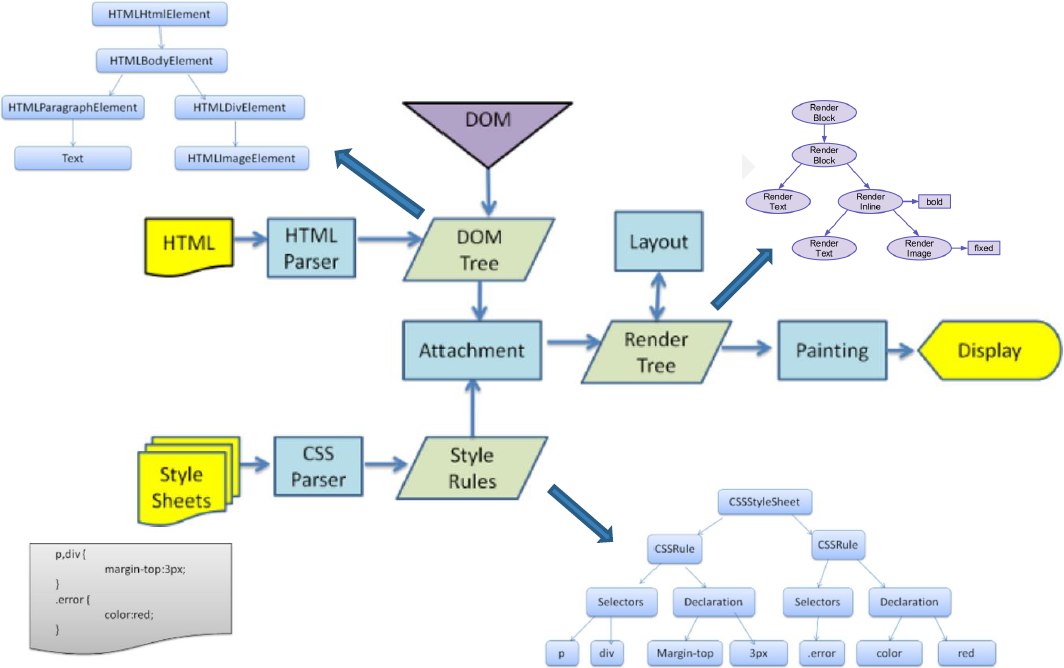
\includegraphics[width=\linewidth]{Images/Rendering_engine_basic_flow.png}
    \caption{Rendering engine basic flow}
    \label{fig:rendering_engine_basic_flow}
\end{figure}

\begin{figure}
    \centering
    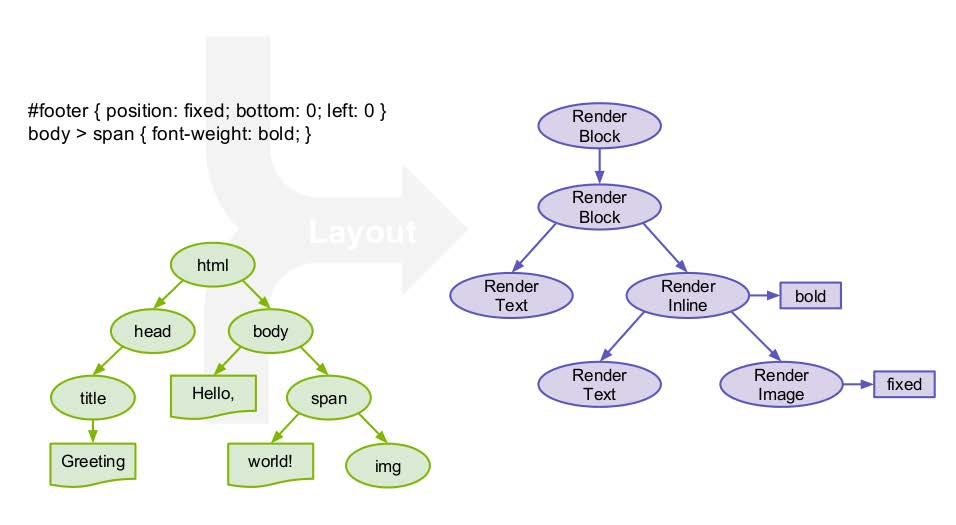
\includegraphics[width=\linewidth]{Images/Render_tree.jpg}
    \caption{Render tree}
    \label{fig:render_tree}
\end{figure}

\section{Rendering Engines}

A rendering engine is the core component of a web browser responsible for
interpreting web content (HTML, CSS, XML) and transforming it into a visual
representation displayed on the screen. Different browsers adopt different
rendering engines, each with its own internal architecture and design choices.

\subsection{Gecko}

\begin{figure}
    \centering
    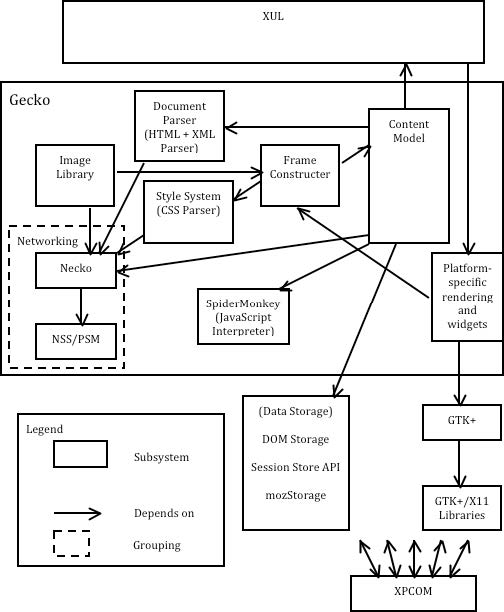
\includegraphics[width=0.5\linewidth]{Images/Gecko_rendering_engine.jpg}
    \caption{Gecko rendering engine architecture}
    \label{fig:gecko}
\end{figure}

Gecko is the rendering engine developed by Mozilla and used primarily in
Firefox-based browsers. It is designed to be modular and standards-compliant,
supporting a wide range of web technologies.

The main components of the Gecko rendering engine include:

\begin{itemize}
    \item \textbf{Style System:} Responsible for parsing CSS stylesheets and
    computing the final styles applied to DOM elements. It retrieves CSS data
    through the networking component (Necko).

    \item \textbf{Image Library:} Manages the loading and decoding of image
    resources. It interacts with Necko to fetch image data from the network.

    \item \textbf{Content Model:} Represents the internal structure of web
    documents and coordinates interactions among the various Gecko components.

    \item \textbf{Frame Constructor:} Builds the frame tree by combining DOM
    structure and computed styles. This step prepares all the necessary
    information before sending the rendered page to the display backend.
\end{itemize}

Gecko emphasizes strict standards compliance and separates concerns such as
networking, parsing, layout, and rendering into well-defined subsystems.

\subsection{WebKit}

\begin{figure}
    \centering
    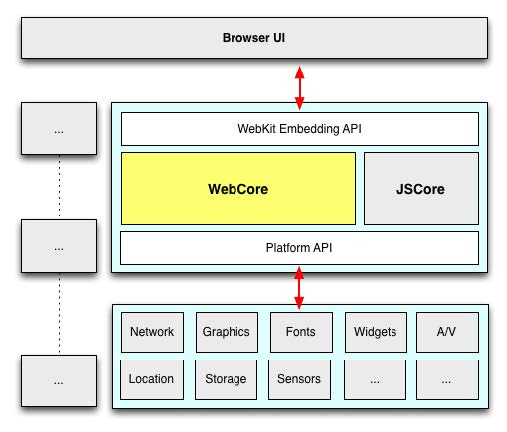
\includegraphics[width=0.5\linewidth]{Images/Webkit_rendering_engine.jpg}
    \caption{WebKit rendering engine architecture}
    \label{fig:webkit}
\end{figure}

WebKit is an open-source rendering engine originally developed by Apple and
later adopted by several browsers and platforms, including Safari and early
versions of Chrome. It provides both rendering capabilities and a JavaScript
engine.

The architecture of WebKit is composed of the following main elements:

\begin{itemize}
    \item \textbf{WebKit Embedding API:} Acts as an interface between the
    rendering engine and the browser user interface, allowing WebKit to be
    integrated into different applications.

    \item \textbf{WebCore:} Contains the core application logic of the rendering
    engine. It handles resource loading, HTML and CSS parsing, layout
    computation, style resolution, painting, event handling, editing features,
    and bindings to JavaScript.

    \item \textbf{JavaScript Engine:} WebKit can use either JavaScriptCore or,
    in some implementations, V8. The JavaScript engine parses and executes
    scripts and allows manipulation of the DOM.
\end{itemize}

WebKit has been widely ported to multiple platforms, each using different
graphics, networking, font, and JavaScript subsystems depending on the target
environment.

\subsection{Blink}

Blink is a rendering engine developed as part of the Chromium project. It was
created as a fork of WebKit's WebCore component and is currently used by many
modern browsers.

Blink is adopted by:
\begin{itemize}
    \item Google Chrome (from version 28)
    \item Opera (version 15 and later)
    \item Microsoft Edge (from 2019)
    \item Amazon Silk
    \item Chromium-based browsers
    \item Android WebView (from Android 4.4)
    \item Qt WebEngine
\end{itemize}

As a fork of WebKit, Blink retains a similar high-level structure but evolves
independently. It focuses on performance optimization, security improvements,
and tighter integration with the Chromium multi-process architecture. \\

Blink works closely with the V8 JavaScript engine and the Chromium networking
stack, enabling efficient execution of web applications and consistent behavior
across platforms.

\section{A Survey of Major Rendering Engines}

Different browsers use different rendering engines, though many modern browsers share engines due to open-source collaboration and software forking. Table ~\ref{tbl:major_rendering_engines} summarizes the major rendering engines in use today. \\

\begin{table}[h]
    \centering
    \begin{tabular}{|l|l|l|}
    \hline
    \textbf{Engine} & \textbf{Associated Browser(s)} & \textbf{Open Source} \\
    \hline
    \textbf{Blink} & Chrome 28+, Edge (2019+), Opera 15+ & Yes \\
    \hline
    \textbf{Gecko} & Firefox & Yes \\
    \hline
    \textbf{WebKit} & Safari, Chrome (pre-28), Android Browser & Yes \\
    \hline
    \textbf{Trident} & Internet Explorer (Legacy) & No \\
    \hline
    \textbf{KHTML} & Konqueror & Yes \\
    \hline
    \end{tabular}
    \caption{Major Rendering Engines}
    \label{tbl:major_rendering_engines}
\end{table}

It is noteworthy that many of these engines share a common lineage. \textbf{Blink}, the engine for Chrome, is a fork of \textbf{WebKit}, which is used by Safari. WebKit, in turn, was originally a fork of \textbf{KHTML}, the engine for the Konqueror browser. This history highlights the importance of open-source development in the browser ecosystem. With the page rendered, the next consideration is how browsers execute the advanced client-side logic that defines modern web applications.

\chapter{Evolution of Client-Side Programmability}

The web has undergone a strategic transformation from a repository of static, hyperlinked documents to a platform for rich, interactive applications. This shift has been driven by the evolution of technologies designed to execute complex code directly on the client-side—within the browser itself. This progression has moved from proprietary, insecure plugins to a standardized, high-performance virtual machine built for the modern web.

\section{The Era of Plugins and Proprietary Extensions}

In the early days of the interactive web, browsers relied on third-party technologies to provide functionality beyond what HTML and early JavaScript could offer. Browser \textbf{plugins} like Adobe Flash and Microsoft Silverlight, along with Microsoft's \textbf{ActiveX} technology, served this purpose. They allowed developers to embed pre-compiled, native code components directly into web pages to enable features such as complex animations, video playback, and rich application interfaces. \\

However, these technologies were beset with problems that ultimately led to their decline. The primary reasons for their deprecation were significant \textbf{performance and security concerns}. By embedding external, native code, these plugins expanded the attack surface of the browser, creating numerous vulnerabilities that could be exploited by malicious actors. They were also resource-intensive, particularly on emerging mobile devices, leading to poor performance and battery life. As a result, the industry moved to phase them out in favor of safer, web-native standards.

\section{WebAssembly: Native-Like Performance on the Web}

The modern, standardized successor to the plugin model is \textbf{WebAssembly (Wasm)}. It was created to solve the same fundamental problem—enabling high-performance applications on the web—but in a way that is secure, efficient, and part of the open web platform.

\subsection{What is WebAssembly?}

WebAssembly is a binary instruction format for a stack-based virtual machine that runs inside the browser. It is not a programming language meant to be written by hand; rather, it is a portable \textbf{compilation target}. This means that code written in high-performance languages like C, C++, and Rust can be compiled into a compact Wasm binary format. This binary can then be downloaded and executed by the browser at near-native speed, far surpassing the performance limitations of even highly optimized JavaScript for CPU-intensive tasks.

\subsection{Goals and Security Considerations}

WebAssembly was designed with several core goals in mind to address the shortcomings of previous technologies:

\begin{itemize}
    \item \textbf{Efficient and Fast:} To be encoded in a size-efficient binary format for fast downloading and to execute at near-native speed by leveraging common hardware capabilities.
    \item \textbf{Safe:} To run within a memory-safe, sandboxed execution environment inside the browser. This sandboxing is critical, as it enforces the browser's security policies and prevents Wasm code from accessing arbitrary system resources.
    \item \textbf{Open and Debuggable:} To be a fully open and standardized part of the web platform. It also includes a human-readable text format (\texttt{.wat}) that aids in debugging, testing, and understanding the compiled code.
\end{itemize}

Despite its powerful capabilities, WebAssembly has not yet achieved universal adoption for all use cases. A primary reason is that, like the plugins it was designed to replace, introducing a new execution environment inherently increases the attack surface of the browser. Although designed with a strong security model, the potential for discovering new vulnerabilities in its implementation remains a concern, leading to a cautious but steady adoption for specific, high-performance applications.

\chapter{Other Core Browser Components}

Beyond the rendering engine, several other critical components are essential for a complete and functional browsing experience.

\begin{itemize}
    \item \textbf{JavaScript Interpreter:} This component is responsible for parsing and executing JavaScript code embedded in a webpage. Its primary function is to enable dynamic page behavior, most notably through DOM manipulation—adding, removing, or modifying elements and styles in real-time. Historically, pure interpreters were slow, as they had to process the same instructions repeatedly within loops or functions. Modern browsers have overcome this limitation by incorporating a \textbf{Just-In-Time (JIT) Compiler}. A JIT compiler identifies sections of code that are executed frequently and compiles them into faster native machine code at runtime (See figure ~\ref{fig:jit_code_compilation}). This approach dramatically improves the performance of complex web applications. Key JIT-enabled JavaScript engines include \textbf{V8} (Chromium), \textbf{SpiderMonkey} (Firefox), and \textbf{Nitro} (Safari).

    \begin{figure}
        \centering
        
\includegraphics[width=\linewidth]{Images/JIT_compiler.jpg}
        \caption{JIT compiles part of the code into faster native machine code}
        \label{fig:jit_code_compilation}
    \end{figure}
    
    \item \textbf{Networking:} The networking component handles all network communication for the browser. It is responsible for retrieving resources from URLs using protocols like HTTP and, in some cases, FTP. Its duties extend to managing the presentation layer of the OSI stack, where it translates between different character sets and resolves MIME media types to understand the format of incoming files. This component also manages a local cache of recently retrieved resources to minimize network traffic and speed up subsequent page loads.
    
    \item \textbf{Display Backend:} The display backend acts as an interface to the operating system's graphical primitives, providing the tools needed to draw windows, UI widgets, and fonts. A significant modern innovation in this area is \textbf{hardware acceleration}. In this model, each render object in the render tree is treated as a separate graphic layer, which is then uploaded to the Graphics Processing Unit (GPU) as a texture. The GPU can then composite these layers and perform transformations (like resizing or rotating) with high performance and minimal impact on the CPU. While powerful, this approach has a potential drawback on resource-constrained mobile devices, where loading an excessive number of textures into the GPU's dedicated memory can lead to performance issues or even crashes.
    
    \item \textbf{XML Parser:} This is a dedicated parser for processing XML documents. Its primary importance in modern web development is enabling the \textbf{AJAX (Asynchronous JavaScript and XML)} programming paradigm. AJAX allows a webpage to make additional HTTP requests to a server to fetch data (often, but not exclusively, in XML format) without requiring a full page reload. This data can then be used to dynamically update parts of the page, creating the seamless, interactive experience characteristic of Rich Internet Applications.
\end{itemize}

Figures ~\ref{fig:internet_explorer_architecture}, ~\ref{fig:google_chrome_architecture} and ~\ref{fig:firefox_architecture} show the architecture of the major modern web browsers which contain the elements exposed in the preceding sections.

\begin{figure}
    \centering
    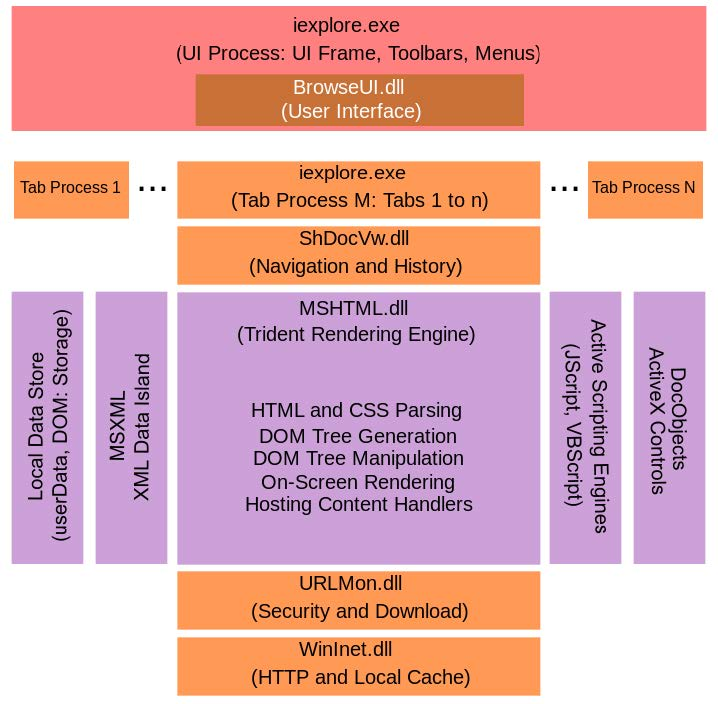
\includegraphics[width=0.5\linewidth]{Images/Internet_Explorer_architecture.jpg}
    \caption{Internet Explorer architecture}
    \label{fig:internet_explorer_architecture}
\end{figure}

\begin{figure}
    \centering
    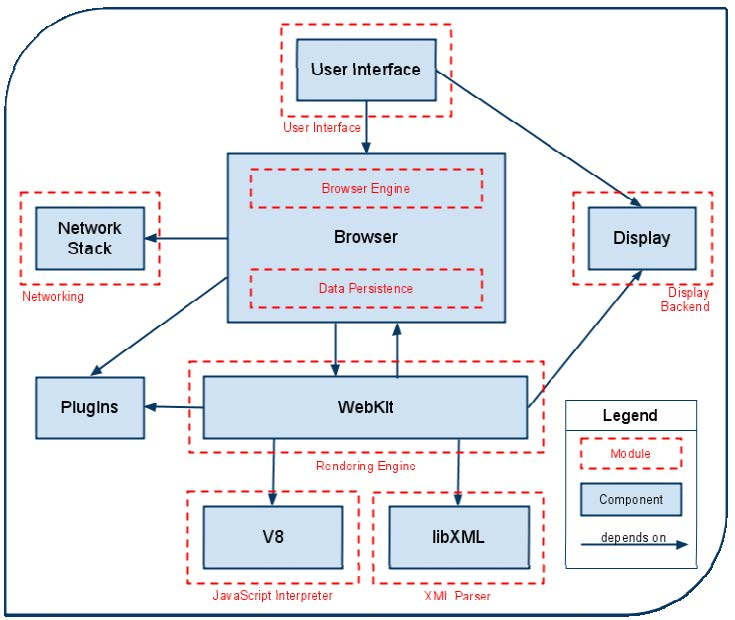
\includegraphics[width=0.5\linewidth]{Images/Chrome_architecture.jpg}
    \caption{Google Chrome architecture}
    \label{fig:google_chrome_architecture}
\end{figure}

\begin{figure}
    \centering
    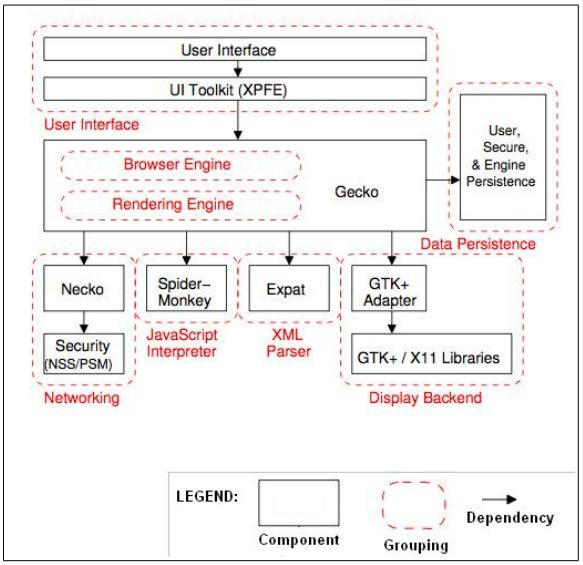
\includegraphics[width=0.5\linewidth]{Images/Firefox_architecture.jpg}
    \caption{Firefox architecture}
    \label{fig:firefox_architecture}
\end{figure}

\chapter{Intermediaries: Optimizing the Client-Server Connection}

\section{Introduction to Web Intermediaries}

While the client-server model is fundamental to the web, the direct communication channel between a browser and an origin server can be augmented by intermediary services. These systems, such as specialized proxy servers and Content Delivery Networks (CDNs), sit between the client and server. They are strategically designed to improve the web experience by enhancing performance, bolstering security, and increasing the scalability of web applications.

\section{Proxy-Based Browsers}

Proxy-based web browsers represent a specific type of intermediary architecture designed to serve web content to resource-constrained devices, such as the first generations of smartphones. (See figure ~\ref{fig:proxy_based_browser}) \\

\begin{figure}
    \centering
    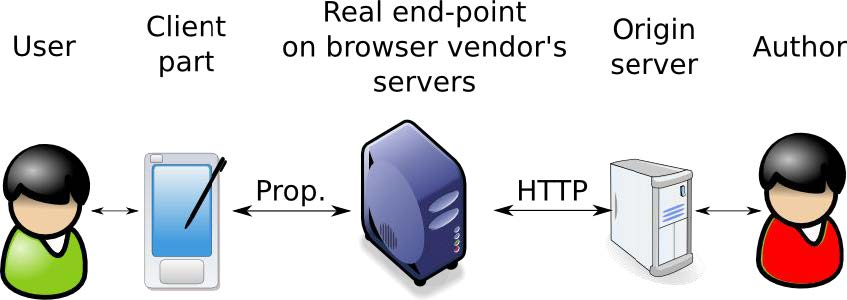
\includegraphics[width=\linewidth]{Images/Proxy-based_browser.jpg}
    \caption{Proxy based browser infrastructure}
    \label{fig:proxy_based_browser}
\end{figure}

In this model, the client device does not communicate directly with the origin server. Instead, the request lifecycle is as follows:

\begin{enumerate}
    \item The client browser sends a page request to the browser vendor's proxy server using a proprietary, optimized protocol.
    \item The proxy server fetches all necessary resources (HTML, CSS, images) from the origin server over a high-bandwidth connection.
    \item The proxy renders the complete page, compresses the output, and encodes it into a single, proprietary resource.
    \item This optimized resource is sent back to the client device, which can process it much more efficiently than the raw source files.
\end{enumerate}

The performance benefits of this model can be analyzed by comparing the formulas for \textbf{turnaround time} ($T$, the total time to load and render a page):

\begin{itemize}
    \item \textbf{Standard Browser:} $T = L_{cs} + T_{cs} + S + C$ (See figure ~\ref{fig:client_server_turnaround})
    \begin{itemize}
        \item $L_{cs}$: Latency between client and source server. (Referring to the empty client request and server response -- In this text we use $L_{cs}$ to denote the whole latency. We could have used a different notation to refer to the  latency of the single messages and, in such case, we would have had $2 \cdot L_{cs}$ in the formula.)
        \item $T_{cs}$: Data transfer time from source to client (Referring to the payload of the server response).
        \item $S$: Server processing time.
        \item $C$: Client processing time (parsing and rendering).
    \end{itemize}
    
    \item \textbf{Proxy-Based Browser:} $T' = L_{cp} + L_{ps} + T_{cp} + T_{ps} + P + S + C'$ (See figure ~\ref{fig:client_proxy_server_turnaround})
    \begin{itemize}
        \item $L_{cp}$, $L_{ps}$: Latency for client-proxy and proxy-source connections (Referring to the empty requests and responses).
        \item $T_{cp}$, $T_{ps}$: Data transfer times for client-proxy and proxy-source (Referring to the payload of the responses).
        \item $P$: Proxy server processing time.
        \item $C'$: Client processing time for the pre-encoded format.
    \end{itemize}
\end{itemize}

\begin{figure}
    \centering
    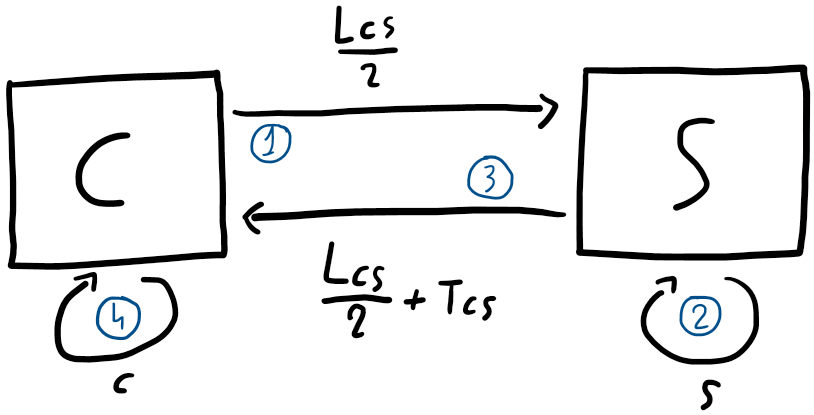
\includegraphics[width=\linewidth]{Images/Client_server_turnaround.png}
    \caption{Client-server turnaround -- The sequence of steps is highlighted in blue.}
    \label{fig:client_server_turnaround}
\end{figure}

\begin{figure}
    \centering
    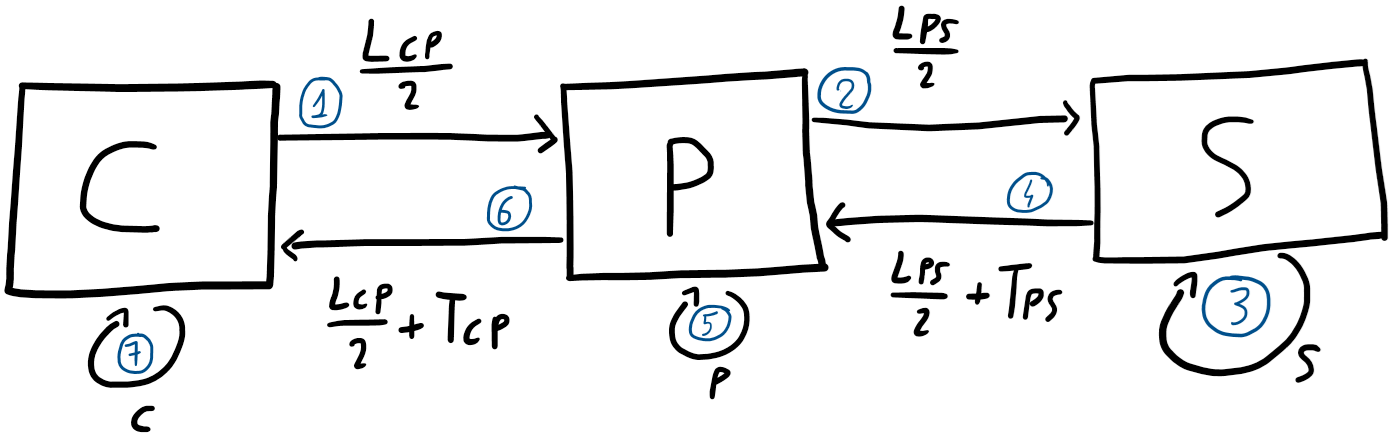
\includegraphics[width=\linewidth]{Images/Client_proxy_server_turnaround.png}
    \caption{Client-proxy-server turnaround -- The sequence of steps is highlighted in blue.}
    \label{fig:client_proxy_server_turnaround}
\end{figure}

The proxy model aims to minimize the total time $T'$ by optimizing each component:

\begin{itemize}
    \item Geographically distributed proxy servers reduce overall latency ($L$) by reducing the latency for client-proxy and proxy-source connection with respect to the latency for the direct client-server connection ($L_{cp}, L_{ps} \ll L_{cs}$).
    
    \item The proxy's high-bandwidth connections and caching reduce the server-to-proxy transfer time with respect to the direct client-server transfer time ($T_{ps} \ll T_{cs}$).
    
    \item Data compression significantly reduces the proxy-to-client transfer time with respect to the direct client-server transfer time ($T_{cp} \ll T_{cs}$). For instance, a page composed of ten resources totaling 1 MB might be consolidated and compressed by the proxy into a single resource of just 100 kB, drastically reducing $T_{cp}$ relative to $T_{cs}$.
    
    \item Pre-encoding the page into a more rapidly processable format reduces the client-side processing effort ($C' < C$).

    \item The proxy processing time ($P$) is small because the proxy has great computational power.
\end{itemize}

\section{Case Study: Cloudflare as a Modern Content Delivery Network}

Cloudflare is a prominent modern example of a web intermediary, operating at a massive scale. It provides a suite of services including a \textbf{Content Delivery Network (CDN)}, a \textbf{reverse proxy}, and comprehensive cybersecurity. As of January 2025, Cloudflare's security services protect approximately 20\% of all websites on the internet. \\

Cloudflare's architecture extends the core principles of proxy-based browsers—optimizing the path between the user and the content—to any website on a global scale. Its key offerings can be categorized as follows:


\begin{itemize}
    \item \textbf{Performance Enhancement:} Cloudflare's vast global network acts as a CDN, caching static content in data centers physically closer to end-users. This practice, known as \textbf{Edge Computing}, dramatically reduces latency and accelerates page load times. Services like \texttt{Cloudflare Workers} even allow developers to run serverless code directly at the edge, further minimizing delays.
    \item \textbf{Security and Protection:} As a reverse proxy, Cloudflare sits in front of the origin server and absorbs malicious traffic before it can cause harm. It is a leading provider of \textbf{DDoS mitigation}. In February 2023, for example, Cloudflare reported blocking the largest HTTP DDoS attack on record, which peaked at 71 million requests per second, demonstrating the sheer scale of its protective capabilities. Its \textbf{"Project Galileo"} initiative provides these vital protection services for free to at-risk public interest groups, journalists, and activists. Additionally, its \textbf{Web Application Firewall (WAF)} and bot management services provide a crucial layer of security against application-level threats.
\end{itemize}

The architecture of the modern web is thus a dynamic ecosystem defined by the holistic interaction of its three core pillars: sophisticated client-side applications like web browsers that render complex content; highly configurable server-side platforms like Apache that provide that content with precision; and powerful network intermediaries like Cloudflare that optimize and secure the connection between them. Together, these components deliver the high-performance, resilient, and secure user experience that defines today's internet.

\end{document}
